
\documentclass[../../main.tex]{subfiles}


\begin{document}
\graphicspath{{../../images/}{images/}} 
\problem{7.2}

\begin{wts}
    The Riesz-Markov-Kakutani Representation Theorem. If (for every) $I$ is a positive linear functional on $\cc{X}$, then there exists a unique Radon measure $\mu$ on $X$, such that
    \[
    I(f) = \int fd\mu
    \]
    for every $f\in\cc{X}$. $\mu$ also satisfies, for every open $U$, and every compact $K\subseteq X$
    \begin{equation}\label{open approximated by If}
        \mu(U) = \sup\left\{I(f),\:f\in\cc{X},\:f\prec U\right\}
    \end{equation}
    \begin{equation}\label{compact approximated by If}
        \mu(K)=\inf\left\{I(f),\:f\in\cc{X},\:f\geq\chi_K\right\}
    \end{equation}
\end{wts}
\providecommand{\borel}{\mathbb{B}_{\Tau}} %Borel generated from Tau
\providecommand{\mustar}{\mu^*} %mu star for outer measure
%
For the sake of completeness, we place the definitions for a Radon measure. Let $X$ be a LCH space, and $\borel$ be its usual $\sigma$-algebra, a measure $\nu$ is a Radon measure iff
\begin{enumroman}
    \item $\nu(K)<+\infty$ for every compact $K$.
    \item $\nu$ is outer-regular on all Borel sets $E$,
    \[
    \nu(E) = \inf\left\{\nu(U),\: U\supseteq E,\:U\in\Tau\right\}
    \]
    Intuition: approximation by open supersets.
    \item $\nu$ is inner-regular on all open sets $U\in\Tau$,
    \[
    \nu(U) = \sup\left\{\mu(K),\: K\subseteq U,\:K\text{ compact}\right\}
    \]
    Intuition: approximation by compact subsets 
\end{enumroman}
%
%
The main proof is extremely long, so we will divide it into several parts. Following Folland's argumentation closely, we will prove (in order)
%
%
\begin{enumalpha}
    \item If $\mu_1$, $\mu_2$ are Radon measures on $X$ such that for every $f\in\cc{X}$
    \[
    \int fd\mu_1=I(f)=\int fd\mu_2
    \]
    then $\mu_1$, $\mu_2$ must satisfy \eqref{open approximated by If}, and $\mu_1 =\mu_2$ on $\borel$.
    \label{7.2.a}
%
%
    \item If we define, for every open set $U$, define $\mu:\Tau\to[0,+\infty]$ such that
    \begin{equation}\label{mu definition on open sets}
    \mu(U) = \sup\left\{I(f),\:f\in\cc{X},\:f\prec U\right\}
    \end{equation}
    Then $\mu$ is countably subadditive, meaning for every $U\in\Tau$, $\{U_{j\geq 1}\}\subseteq \Tau$
    \[
    U = \bigcup U_{j\geq 1}\implies \mu(U)\leq \sum\mu(U_{j\geq 1})
    \]\label{7.2.b}
%
%
    \item $\mu(\varnothing)=0$, $\{\varnothing, X\}\subseteq \Tau$, so that by Theorem 1.10 $\mu$ induces an outer-measure $\mu^*$
    
    \begin{equation}\label{mustar outermeasure def}
        \mu^*(E)= \inf\left\{\sum \mu(U_{j\geq 1}),\:U_j\in\Tau,\:E\subseteq\bigcup U_{j\geq 1}\right\}
    \end{equation}
    \label{7.2.c}
%    
%    
    \item If $\mu^*$ is as described above, then if $\mu$ is countably subadditive on $\Tau$, then
    \begin{equation}\label{mustar outer regularity on Borel Sets}
        \mu^*(E) = \inf\left\{\mu(U),\:U\supseteq E,\: U\in\Tau\right\} 
    \end{equation}
    Meaning the two definitions in \eqref{mustar outermeasure def} and \eqref{mustar outer regularity on Borel Sets} are equal.
    \label{7.2.d}
%
%
    \item $\mustar$ and $\mu$ agree on all open sets, and $\mustar|_\Tau = \mu$, 
    \label{7.2.e}
%
%    
    \item Using again the definition in \eqref{mustar outermeasure def} and \eqref{mustar outer regularity on Borel Sets}, we show that every open set $U\in\Tau_X$ is $\mustar$-measurable, meaning for every $E\subseteq X$,
    \[
    \mustar(E) = \mustar(E\cap U) + \mustar(E\setminus U)
    \]
    With this, since the set of all outer-measurable ($\mustar$-measurable) sets, $\mathcal{M}^*$ form a $\sigma$-algebra, 
    \[
    \Tau\subseteq \mathcal{M}^*\implies \borel\subseteq\mathcal{M}^*
    \]
    By Theorem 1.1, and define 
    \begin{equation}\label{mu borel extension}
        \mu = \mustar|_{\borel}
    \end{equation} 
    is a Borel measure. And we note in passing that $\mu$ is outer-regular on all $E\in\borel$,
    \begin{equation}\label{mu outer-regular on all Borel}
         \mu(E) = \inf\left\{\mu(U),\:U\supseteq E,\: U\in\Tau\right\} 
    \end{equation}
    \label{7.2.f}
%
%
    \item Using \eqref{mu borel extension} for the definition of  $\mu$ on $\borel$, we prove that
    \begin{itemize}
        \item $\mu$ is outer-regular on all Borel sets, and
        \item $\mu$ satisfies Equation \eqref{open approximated by If}.
    \end{itemize}
    \label{7.2.g}
%
%
    \item $\mu$ satisfies Equation \eqref{compact approximated by If}
    \label{7.2.h}
%
%
    \item $\mu$ is finite on all compact sets.
    \label{7.2.i}
%
%
    \item $\mu$ is inner-regular on all open sets.
    \label{7.2.j}
%
%
    \item For every $f\in\cc{X,[0,1]}$, 
    \begin{equation}\label{integral equation}
        I(f) = \int fd\mu
    \end{equation}
    \label{7.2.k}
%
%
    \item For every $f\in\cc{X}$,
    \begin{equation}\label{integral equation general}
        I(f) = \int fd\mu
    \end{equation}
\end{enumalpha}
%Lemma

A small lemma needs to be made before proceeding, that concerns the 'monotonicity' of $I$ on $C_c{X}$.
    \begin{lemma}\label{lemma I is monotonic}
        Suppose that $f,\, g\in\cc{X}$, and $f\geq g\geq 0$ for every $X$, then $f-g\in\cc{X}$ and $I(f)\geq I(g)$
    \end{lemma}
    \begin{proof}
        Suppose that $x\in X$ where $f(x) = 0$, then
        \[
        f(x)-g(x) = -g(x)\geq 0\implies g(x)=0\implies f-g=0
        \]
        Hence
        \begin{align*}
            \left\{x,\:f(x)=0\right\}\subseteq\left\{x,\:f(x)-g(x)=0\right\}&\implies \left\{x,\:f(x)-g(x)\neq0\right\}\subseteq \left\{x,\:f(x)\neq0\right\}\\
            &\implies \supp{f-g}\subseteq \supp{f}
        \end{align*}
        Since $\supp{f}$ is compact, and $\supp{f-g}$ is a closed subset of $\supp{f}$, yields $f-g\in\cc{X}$. And if $I$ is any positive linear functional on $\cc{X}$, then
        \begin{align*}
            f-g\geq 0&\implies I(f-g)\geq 0\\
            &\implies I(f)\geq I(g)\geq 0
        \end{align*}
    \end{proof}
    %End of Lemma proving monotonicity.
\remark If $f\prec U$ and $g\prec U$ for some open subset $U\subseteq X$, then clearly $\supp{f-g}\subseteq \supp{f}\subseteq U$, and $1\geq f\geq f-g\geq 0$ means that $f-g\prec U$ as well.

\subsubsection{Part a}
\begin{proof}
    Suppose that $\mu_1$ and $\mu_2$ are Radon measures on $X$, and for every $f\in\cc{X}$,
    \[
    \int fd\mu_1 = I(f) = \int fd\mu_2
    \]
    We first prove \eqref{open approximated by If}. Without loss of generality, by monotonicity of $L^+$, if $f\prec U$ for some open $U$, then $0\leq f\leq \norm{f}_u\chi_U=\chi_U$ for all $x$ and
    \[
    \int fd\mu_1\leq \int \norm{f}_u\,\chi_U\:d\mu_1 \leq \mu_1(U)
    \]
    Therefore $\mu_1(U)$ (resp. $\mu_2(U)$) is an upper-bound for the set
    \[
    \left\{I(f),\:f\in\cc{X},\:f\prec U\right\}
    \]
    Since $\mu_1$ is inner-regular on $U\in\Tau$, for every $\varepsilon>0$ we can find some compact $K\subseteq U$ where
    \[
    \mu_1(U)-\varepsilon<\mu_1(K)
    \]
    By Urysohn's Lemma (Theorem 4.32), there exists some $g\in\cc{X}$ with
    \begin{itemize}
        \item $g\in\cc{X,[0,1]}$,
        \item $g=1$ on $K\subseteq U$,
        \item $g=0$ outside some $\overline{V}\subseteq U$, and
        \item $g\prec U$.
    \end{itemize}
    Hence for every $x\in K$, $g\geq \chi_K$. If $x\notin K$ then $g\geq 0 = \chi_K$; so $g-\chi_K\geq 0$ for every $x\in X$. Since $\chi_K\prec U$, using Lemma \ref{lemma I is monotonic}, we get
    \[
    \mu_1(K)\leq \int\,\chi_K\:d\mu_1=I(\chi_K)\leq I(g)
    \]
    So for every $\varepsilon>0$, there exists a $g\in\cc{X}$, and $g\prec U$ where
    \[
    \mu_1(U)-\varepsilon<\mu_1(K)\leq I(g)
    \]
    Therefore $\mu_1(U) = \sup\left\{I(f),\:f\in\cc{X},\:f\prec U\right\}$, and the first claim in \ref{7.2.a} is proven. To show that $\mu$ is indeed unique, since for every open set $U$, we must have $\mu_1(U)=\mu_2(U)$, and if $E\in\borel$ is any Borel set, and by outer-regularity,
    \[
    \mu_1(E) = \inf\left\{\mu_1(U), U\supseteq E, U\in\Tau\right\} = \inf\left\{\mu_2(U), U\supseteq E, U\in\Tau\right\}=\mu_2(E)
    \]
    Therefore this measure is unique.
\end{proof}
%
%
\subsubsection{Part b}
\begin{proof}
To show countable subadditivity for $\mu$ with equation \eqref{mu definition on open sets}, fix any $U\in\Tau$ and a sequence $\{U_{j\geq 1}\}\subseteq \Tau$ with $U = \bigcup U_{j\geq 1}$. It suffices to show that the partial sum of $\sum \mu(U_{j\leq n})$ is greater than $I(f)$ for any $f\in\cc{X},\:f\prec U$ (hence it is an upper bound).\\

Fix any $f$, then denote $K=\supp{f}\subseteq U$, and since $\{U_{j\geq 1}\}$ is an open cover for $K$, there exists a finite subcollection, $B\subseteq\nat^+$ such that 
\[
K\subseteq \bigcup_{j\in B}U_j
\]
Using Theorem 4.41 on this finite cover of $K$, there exists a partition of unity in $\{g_{j\leq n}\}$ where
\begin{itemize}
    \item $g_j\in\cc{X,[0,1]}$,
    \item $g_j\prec U_j\subseteq U$ for every $j\leq n$, and
    \item $\sum g_j=1$ on $K$,
\end{itemize}
And notice for every $j\leq n$, 
\begin{align*}
    \{f=0\}\cup\{g_j=0\}\subseteq \{f\cdot g_j=0\}&\implies\{f\cdot g_j\neq 0\}\subseteq \{f\neq 0\}\cap \{g_j\neq 0\}\\
    &\implies \supp{f\cdot g_j}\subseteq \supp{f}\cap \supp{g_j}\\
    &\implies \supp{f\cdot g_j}\subseteq U_j\subseteq U
\end{align*}
Hence $f\cdot g_j\prec U$ and $f\cdot g_j\in\cc{X,[0,1]}$ for every $1\leq j\leq n$. Moreover, if we take the sum over a finite $n$, we obtain $f = \sum f\cdot g_{j\leq n}$, this is because for every $x\in X$, so we have 
\[
\sum_{j\leq n}f(x)\cdot g_j{x} = f(x)\cdot\sum_{j\leq n}g_j(x) = f(x)
\]
Then $I(f) = I(\sum f\cdot g_j) = \sum I(f\cdot g_j)$. And by definition of $\mu(U_j)$, since it is the supremum over all $I(h_j)$, where $h_j\in\cc{X,[0,1]}$ and $h_j\prec U_j$
\[
I(f\cdot g_j)\leq \mu(U_j),\quad \forall j\leq n
\]
Hence
\[
I(f)\leq \sum_{j\leq n} \mu(U_j)\leq \sum_{j\geq 1}\mu(U_j)
\]
Where for the last estimate we used the fact that $\mu$ is non-negative, and since this holds for any $f$, we can conclude that $\mu(U)\leq \sum_{j\geq 1} \mu(U_j)$.
\end{proof}

\subsubsection{Part c}
\begin{proof}
    By definition of a topology, $\{\varnothing, X\}\subseteq \Tau$, and $\mu(\varnothing) = \sup\{I(f),\: f\in\cc{X},\:f\prec \varnothing\}$, so $\supp{f}=\varnothing$, and $\{x,\:f(x)\neq 0\}\subseteq\varnothing$, so the set contains one element, namely $I(0)=0$ by linearity. So $\mu(\varnothing)=0$. The assumptions for Theorem 1.10 are satisfied and \eqref{mustar outermeasure def} is indeed an outer-measure.
\end{proof}

\subsubsection{Part d}
\begin{proof}
    Denote the right members of \eqref{mustar outermeasure def} and \eqref{mustar outer regularity on Borel Sets} by $W_1$ and $W_2$, we wish to show that $\inf{W_1} = \inf{W_2}$. Clearly $\inf{W_1}\leq \inf{W_2}$, since $W_2\subseteq W_1$. Now, if $\mu$ is countably additive, then for every $\omega\in W_1$ induces a sequence of open sets $\{U_{j\geq 1}\}$ such that $E\subseteq \bigcup U_{j\geq 1}$. Denote the union over $\{U_{j\geq 1}\}$ by $U$, which is also another open set, 
    \[
    \inf{W_2}\leq\mu(U)\leq \sum \mu(U_{j\geq 1})=\omega
    \]
    Since $\omega$ is arbitrary, we conclude that $\inf{W_2}=\inf{W_1}$, and this proves \ref{7.2.d}.
\end{proof}
\subsubsection{Part e}
\begin{proof}
    If $U$ and $V$ are open subsets of $X$, and if $U\subseteq V$, then
    \begin{align*}
        U\subseteq V &\implies\left\{f\in\cc{X},\:f\prec U\right\}\subseteq\left\{f\in\cc{X},\:f\prec V\right\} \\
        &\implies \left\{I(f),\:f\in\cc{X},\:f\prec U\right\}\subseteq\left\{I(f),\:f\in\cc{X},\:f\prec V\right\}
    \end{align*}
    Hence $\mu(U)\leq \mu(V)$. Now by equation \eqref{mustar outer regularity on Borel Sets}, $\mustar(U)\leq \mu(U)$. To show the reverse inequality, suppose by contradiction that $\mustar(U)<\mu(U)$.\\
    
    Since $\mustar(U)$ is an infimum, then for every $\varepsilon>0$ there exists some $V\supseteq U$ where if we write $\mustar(U)+\varepsilon=\mu(U)$
    \[
    \mu(V)<\mustar(U)+\varepsilon=\mu(U)\implies \mu(V)<\mu(U),\:U\subseteq V
    \]
    This contradicts what we have just proven, and therefore $\mustar(U)=\mu(U)$ for every open set $U$.
\end{proof}
\subsubsection{Part f}
\begin{proof}
We wish to show that every open set $U$ is $\mustar$-measurable. By Theorem 1.10, it suffices to show that for every $E\subseteq X$
\begin{equation}\label{mustar measurable}
\mustar(E) \geq \mustar(E\cap U) +\mustar(E\setminus U)
\end{equation}
because the reverse inequality is given by subadditivity of $\mustar$, and we can also assume that $\mustar(E)<+\infty$. Let us assume that $E$ is open, we wish to find some function $h\in\cc{X},\: h\prec E$ with
\[
I(h)> \mustar(E\cap U) + \mustar(E\setminus U) - 2\varepsilon
\]
The above formula is fussy, but the liberty is taken to show it beforehand to avoid any potential confusion that follows. Since $E\cap U$ is an open subset of $X$, the definition of $\mu(E\cap U) = \mustar(E\cap U)$ in \eqref{mu definition on open sets} tells us that every $\varepsilon>0$ induces some $f\in\cc{X},\:f\prec E\cap U$ where
\begin{equation}\label{If part f}
    I(f)>\mu(E\cap U)-\varepsilon=\mustar(E\cap U)-\varepsilon
\end{equation}
Also, $\supp{f}$ is a closed set (compact subsets of Hausdorff spaces are closed), therefore $E\setminus\supp{f}$ is an open set. We make a small diversion from the current part of the proof and turn out attention to the fact that
\begin{align*}
    \supp{f}\subseteq U&\implies U^c\subseteq (\supp{f})^c\\
    &\implies E\setminus U\subseteq E\setminus\supp{f}
\end{align*}
And because the outer-measure $\mustar$ is monotone,
\begin{equation}\label{mustar motone part f Esuppf}
    \mustar(U)\leq \mustar(E\setminus \supp{f})
\end{equation}
Now, using the definition of $\mu(E\setminus\supp{f})$ (recall that $E\setminus\supp{F}$ is an open set), for every $\varepsilon>0$, there exists some $g\in\cc{X}$, $g\prec E\setminus\supp{F}$ with
\begin{equation}\label{Ig part f}
I(g)>\mu(E\setminus \supp{f})-\varepsilon =\mustar(E\setminus \supp{f})-\varepsilon
\end{equation}
It is at this part of the proof where we wish to define $h=f+g$, but first we must verify
\begin{itemize}
    \item $f+g\in\cc{X,[0,1]}$,
    \item $f+g\prec E$
\end{itemize}
The sum of two non-negative functions is non-negative, and for every $x\in\supp{f}$, $f\leq 1$. Also
\begin{align*}
    \supp{g}\subseteq (\supp{f})^c&\implies\supp{f}\subseteq (\supp{g})^c\\
    &\implies \supp{f}\subseteq \{g=0\}
\end{align*}
The last implication comes from taking complements on both sides of $\{g\neq 0\}\subseteq \supp{g}$. So $x\in\supp{f}\implies f+g\leq 1$. Now if $x\notin\supp{f}$, then $f+g=g\leq 1$. Furthermore, $\supp{f+g}$ is a closed subset of compact $\supp{f}\cup\supp{g}$. This is because $\{f+g\neq 0\}\subseteq \{f\neq 0\}\cup\{g\neq 0\}$, and the finite union of two compact sets is again again compact.\\

A moment's thought should yield the fact that the last estimate should be an equality, but it is a needless distraction. Therefore $\supp{f+g}$ is compact and $f+g\in\cc{X,[0,1]}$.\\

Now both bullet points are satisfied, and we can set $h=f+g$. Adding equation \eqref{Ig part f} with \eqref{If part f} gives us
\[
I(h) = I(f) + I(g) > \mustar(E\cap U)+\mustar(E\setminus \supp{f})-2\varepsilon
\]
Upon applying \eqref{mustar motone part f Esuppf} to the right member of the above estimate, we have
\[
I(h)>\mustar(E\cap U)+\mustar(E\setminus U)-2\varepsilon
\]
But this particular $h\in\cc{X}\cap\{f\prec E\}$, therefore
\[
\mustar(E)\geq I(h)>\mustar(E\cap U)+\mustar(E\setminus U)-2\varepsilon
\]
Since $\varepsilon>0$ is arbitrary, equation \eqref{mustar measurable} holds for every open $E$. Now for any general $E\subseteq X$, fix any $\varepsilon>0$ and by how we defined $\mustar(E)$, there exists some open $V\supseteq E$ —recall that $\mustar(E)$ is the infimum over the set of $\mu(V)$ where $V$ is an open superset of $E$ — hence
\[
\mustar(E)+\varepsilon>\mu(V)\geq\mustar(V\cap U) + \mustar(V\setminus U)
\]
By monotonicity (twice) of the outer-measure $\mustar$, we have
\[
\mustar(E)+\varepsilon>\mustar(E\cap U) + \mustar{E\setminus U}
\]
Let $\varepsilon\to 0$, and we get
\[
\mustar(E)\geq \mustar(E\cap U) + \mustar(E\setminus U)
\]
Therefore every open $U\subseteq X$ is $\mustar$-measurable. So $\mu = \mustar|_{\borel}$ is a Borel measure on $X$.
\end{proof}
\subsubsection{Part g}
\begin{proof}
    To show outer-regularity, fix any $E\in\borel$, then by definition,
    \[
    \mu(E) =\mustar(E)= \inf\left\{\mu(U),\:U\supseteq E,\:U\in\Tau\right\}
    \]
    And for every open $U$, \eqref{open approximated by If} follows from Equation \eqref{mu definition on open sets}.
\end{proof}
\subsubsection{Part h}
\begin{proof}
We want to show that for every compact $K$, Equation \eqref{compact approximated by If} holds. To reduce the notational baggage that follows, we agree to define
\[
\left\{I(f),\: f\in\cc{X},\:f\prec U\right\} = \{I(f),\: f\prec U\}
\]
Similarily for $\{I(f),\: f\geq \chi_K\}$. If $\mu(K)=0$, then $\mu(K)$ is obviously a lower bound, since $f\geq \chi_K\geq 0$ means that $I(f)\geq 0$, for every $f\geq \chi_K$. So we can suppose $\mu(K)>0$.\\

Fix an arbitrary $f\geq \chi_K$, then this particular $f$ induces an open set $U_\alpha=\{f>1-\alpha\}$, where $\alpha>0$. Notice also that
\[
K\subseteq\{f\geq 1\}\subseteq \{f>1-\alpha\}=U_\alpha
\]
Since $U_\alpha$ is an open superset of $K$, by Equation \eqref{mu outer-regular on all Borel}, $\mu(K)\leq \mu(U_\alpha)$, but $\mu(U_\alpha)$ is simply the supremum of $\{I(g),\:g\prec U_\alpha\}$. If we wish to show that $\mu(K)\leq \mu(U_\alpha)\leq I(f)$, it suffices to show that $I(f)$ is an upper-bound for $\{I(g),\:g\prec U_\alpha\}$.\\

Fix any $I(g)\in\{I(g),\:g\prec U_\alpha\}$, note that $1-\alpha\neq 0$ for any $\alpha$ small enough, then 
\begin{itemize}
    \item $f/(1-\alpha)>1$ on $U_\alpha$,
    \item $1\geq g\geq 0$ on $U_\alpha$, in particular, $f/(1-\alpha)-g\geq 0$ on $U_\alpha$,
    \item If $x\notin U_\alpha$, then $f/(1-\alpha)-g = f(1-\alpha)\geq 0$.
    \item Therefore $f/(1-\alpha)-g\geq 0$ for any $x$, and by Lemma \ref{lemma I is monotonic},
    \[
    I(f/(1-\alpha))\geq I(g)\quad\forall g\prec U_\alpha
    \]
\end{itemize}
Combining the above estimate with $\mu(K)\leq \mu(U_\alpha)$ gives us
\[
\mu(K)\leq \dfrac{1}{1-\alpha}I(f)
\]
Now write $\varepsilon = \alpha/\mu(K)>0$ and for every $\varepsilon>0$ we get
\[
\mu(K)-I(f)\leq\alpha\mu(K)=\varepsilon
\]
Send $\varepsilon\to 0$ and $\mu(K)\leq I(f)$ for every $f\geq\chi_K$.\\ 

To show that $\mu(K)$ is indeed the infimum for $\{I(f),\: f\geq \chi_K\}$, notice that for every $\varepsilon>0$ we can obtain some open superset $U\supseteq K$ (by outer-regularity) where $\mu(U)<\mu(K)+\varepsilon$. By Urysohn's Lemma, there exists some $g\prec U$, $g(x)=1$ for every $x\in K$.
\[
g\in \{I(f),\: f\prec U\}\cap\{I(f),\: f\geq\chi_K\}
\]
Therefore $I(g)\leq\mu(U)<\mu(K)+\varepsilon$ as desired, and Equation \eqref{compact approximated by If} holds.
\end{proof}
\subsubsection{Part i}
\begin{proof}
$\mu(K)<+\infty$ for every compact $K$. Indeed, since $I(\chi_K)\in\{I(f),\:f\geq\chi_K\}$, then by Theorem 7.1, there exists a constant $C_K\geq 0$ that bounds
\[
\mu(K)\leq |I(\chi_K)| = I(\chi_K)\leq C_K\cdot \norm{\chi_K} = C_K<+\infty
\]
\end{proof}
\subsubsection{Part j}
\begin{proof}
Fix any open set $U$, then for every $\varepsilon>0$, there exists some $f\prec U$ with $\mu(U)-\varepsilon<I(f)$. Then denote $K=\supp{f}\subseteq U$. If we take any $I(h)\in\{I(h),\:h\geq \chi_K\}$, then $h\geq f$ gives us $I(h)\geq I(f)$ by Lemma \ref{lemma I is monotonic}. So $I(f)$ is a lower bound of $\{I(h),\: h\geq \chi_K\}$, therefore
\[
\mu(U)-\varepsilon\leq I(f)\leq \mu(K)
\]
Since $\supp{f}=K\subseteq U$, this proves inner-regularity of $\mu$ on open sets.
\end{proof}
\subsubsection{Part k}
\begin{proof}
    Suppose $f\in\cc{X,[0,1]}$, we first show that Equation \eqref{integral equation} holds. We divide the interval $[0,1]$ into $N\geq1$ chunks by writing 
    \[
    K_j = \{f\geq j/N\}
    \]
    for every $1\geq j\geq N$. And define $K_0=\supp{f}$. Each $K_j$ is a closed subset of $\supp{f}$, and therefore compact. More is true, 
    \begin{itemize}
        \item $K_{j-1}\supseteq K_j$ for every $1\leq j\leq N$.
        \item $x\in K_j$ iff $f(x)\in \left[\frac{j}{N},\: 1\right]$,
        \item $x\notin K_j$ iff $f(x)\in \left[0,\frac{j}{N}\right)$, and
        \item $x\in (K_{j-1}\setminus K_j)$ iff $f(x)\in \left[\frac{j-1}{N},\:\frac{j}{N}\right)$
    \end{itemize}
    Folland constructs a finite sequence of compactly supported functions, $\{f_j\}$, where $1\leq j \leq N$ such that
    \begin{itemize}
        \item Each $0\leq f_j\leq 1/N$,
        \item If $x\in (K_{m}\setminus K_{m+1})$ iff $f(x)\in\left[\frac{m}{N},\:\frac{m+1}{N}\right)$ means that $f_j=1$ for all $1\leq j\leq m$, and
        \item $f_{m+1} = f-m/N$ on $K_m$, such that 
        \[
        f(x) = \left(\sum f_{j\leq m}(x)\right) + \left(f(x)-\dfrac{m}{N}\right) = \dfrac{m}{N} + \left(f(x)-\dfrac{m}{N}\right)
        \]
        \item And for every $m<j\leq N$, $f_j=0$.
        \item If $x\notin K_m$ iff $f(x)\in\left[0,\:\frac{m}{N}\right)$ then for every $m+1\leq j\leq N,\:f_j=0$.
        
    \end{itemize}
    The illustration for when $N=5$ below should make things clearer.\\
    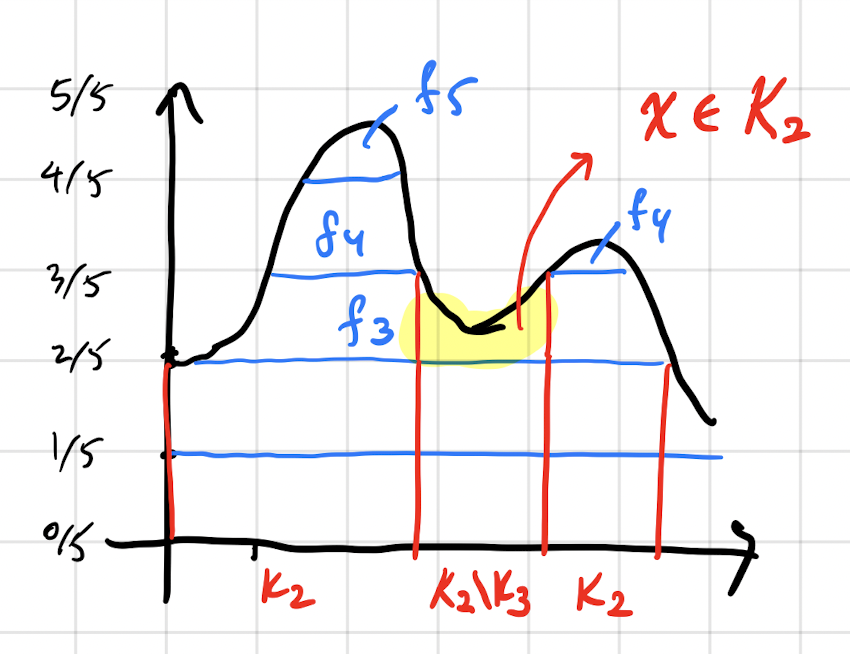
\includegraphics[scale=0.50]{FollandTheorem7_2.png}
    \\ It is also trivial to verify that
    \begin{itemize}
        \item For every $x\in K_j$, $f_j=N^{-1}$, and
        \begin{equation}\label{f_j greater than K j}
        \chi_{K_{j}}N^{-1}\leq f_j
        \end{equation}
        Also, if $x\notin K_j$ then $f_j\geq 0$, therefore $f_j\geq \chi_{K_j}N^{-1}$ at every $x$.
        \item If $x\notin K_{j-1}$ then $f_j = 0\leq \chi_{K_{j-1}}\cdot N^{-1}$. If $x$ is in $K_{j-1}$ then $f_j\leq N^{-1}$ by construction and therefore
        \begin{equation}\label{f_j less than K j-1}
        f_j\leq \chi_{K_{j-1}}N^{-1}
        \end{equation}
        for all $x$.
        \item $f_j\in\cc{X}$, since $\supp{f_j}\subseteq \supp{f}$.
    \end{itemize}
   Combining Equations \eqref{f_j greater than K j} with \eqref{f_j less than K j-1}, and by monotonicity in $L^+(X,\borel,\mu)$, since $f_j\in L^+$
   \[
   \int \dfrac{1}{N}\chi_{K_j}d\mu\leq \int f_jd\mu\leq\int \dfrac{1}{N}\chi_{K_{j-1}}d\mu
   \]
  % 
   And for every $1\leq j\leq N$, 
   \begin{equation}\label{integral fj estimate}
   \frac{1}{N}\mu(K_j)\leq \int f_jd\mu\leq \frac{1}{N}\mu(K_{j-1})
   \end{equation}
   Furthermore, from Equation \eqref{f_j greater than K j}, since $Nf_j\geq \chi_{K_j}$ then by Equation \eqref{compact approximated by If},
    \[
    \mu(K_j)\leq I(N f_j)\implies\dfrac{1}{N}\mu(K_j)\leq I(f_j)
    \]
    Now for any arbitrary $I(h)\in\{I(h),\: h\geq \chi_{K_{j-1}}\}$, since
    \[
    h\geq\chi_{K_{j-1}}\geq N f_j\implies I(h)\geq I(N f_j)
    \]
    So $NI(f_j)$ is a lower bound for $\{I(h),\: h\geq \chi_{K_{j-1}}\}$ and 
    \[
    I(f_j)\leq\dfrac{1}{N}\mu(K_{j-1})
    \]
    Combining the last two results, with $I(f_j)$, we get
    \begin{equation}\label{I fj estimate}
    \dfrac{1}{N}\mu(K_j)\leq I(f_j)\leq\dfrac{1}{N}\mu(K_{j-1})    
    \end{equation}
    Taking the sum over $1\leq j\leq N$ for Equations \eqref{integral fj estimate} and \eqref{I fj estimate}. Define $A = N^{-1}\sum_0^{N-1}\mu(K_j)$, and $B=N^{-1}\sum_1^{N}\mu(K_j)$
    \[
        B\leq \int fd\mu \leq A
    \]
    And also
    \[
        B\leq I(f)\leq A
    \]
    This is because of finite additivity of both $I$ and the integral, and $f = \sum f_j$ on $K_0=\supp{f}$. Subtracting the two equations (keeping in mind that $\mu(K_j)<+\infty$ for any compact $K_j$), we get
    \[
        (-1)(A-B)\leq \left(\int fd\mu - I(f)\right)\leq A-B\implies \left|\int fd\mu - I(f)\right|\leq A-B
    \]
    It is trivial to verify that 
    \[
    0\leq A-B = N^{-1}(\mu(K_0)-\mu(K_N))\leq N^{-1}\mu(K_0)
    \]
    as $K_N\subseteq K_0$. Let $N\to\infty$ and
    \[
    \int fd\mu = I(f)
    \]
    Equation \eqref{integral equation} holds as desired.
\end{proof}

\subsubsection{Part l}
\begin{proof}
Now for any general $f\in\cc{X}$, $f$ must be bounded on the plane since $\cc{X}\subseteq \bc{X}$, and $|f|\leq M_0$ for some $M_0\geq 0$. Since $\supp{f}$ is compact, we know that 
\[
\int |f|d\mu\leq \int M_0\chi_{\supp{f}}d\mu\leq M_0\mu(\supp{f})<+\infty
\]
And $\cc{X}\subseteq L^1(\mu)$. Furthermore,
\[
\frac{1}{2}( |\Re{f}| + |\Im{f}| ) \leq |f|\leq M_0
\]
So that $\Re{f}$ and $\Im{f}$ are in $\cc{X}$. Without loss of generality, we may assume that $f$ is real. Define $f_1 = \Re{f}^+/M_0$ and $f_2 = \Re{f}^-/M_0$ and it immediately follows that $f_1,\,f_2\in\cc{X,[0,1]}$.\\

By linearity of $I$ on $\cc{X}$ and the integral in $L^1(\mu)$, 
\[
I(f_1-f_2) = I(f) = \int fd\mu = \int f_1d\mu - \int f_2d\mu
\]
Then we may apply the above to the real and imaginary parts of a general $f\in\cc{X}$, and this completes the proof.
\end{proof}

\end{document}